\documentclass[12pt]{beamer}

\usepackage{beamerthemesplit}


\usepackage{beamerthemesplit}

\usepackage{beamerStatisticsTAMU} 

\logo{\includegraphics[height=1.5cm]{STAT_Horz-Aggie-Maroon.pdf}\vspace{220pt}}


\usepackage{amsmath}
\usepackage{amssymb}
\usepackage{verbatim}
\usepackage{bibentry}
%\usepackage{biblatex}
%\usepackage{natbib}
\newcommand{\argmin}[1]{\underset{#1}{\operatorname{argmin}}\text{ }}
\newcommand{\argmax}[1]{\underset{#1}{\operatorname{argmax}}\text{ }}
\usepackage{bbm}
\usepackage{bm}
\usepackage[absolute,overlay]{textpos}

\newcommand{\Var}{\text{Var }}
\newcommand{\Cov}{\text{Cov }}
\newcommand{\E}{\mathbb{E}}
\newcommand{\V}[1]{{\bm{\mathbf{\MakeLowercase{#1}}}}} % vector
\newcommand{\M}[1]{{\bm{\mathbf{\MakeUppercase{#1}}}}} % matrix
\newcommand{\todo}[1]{{\color{red}TODO: #1}}

\newcommand{\w}{0.8in}
\newcommand{\h}{1in}
\usepackage{graphicx}
\newcommand{\indep}{\rotatebox[origin=c]{90}{$\models$}}

\newtheorem{assumptions}{Assumptions}

\setbeamertemplate{headline}[default]
\setbeamertemplate{footline}[page number]
\setbeamertemplate{navigation symbols}{}
\setbeamertemplate{bibliography item}[text]

\title{Modeling Variable Star Light Curves}
\author{James Long}
%%\institute{UC Berkeley}
\date{\today}
\begin{document}

\frame{\titlepage}

\frame{\tableofcontents}

\AtBeginSection[]
{
  \begin{frame}<beamer>
    \frametitle{Outline}
    \tableofcontents[currentsection,currentsubsection]
  \end{frame}
}


%%%%%%%%
%%%%%%%% TODO: redo first section with more emphasis on multiband, lomb scargle
%%%%%%%%


\section{Time Domain Astronomy and Variable Stars}

\begin{frame}{Periodic Variable Stars}
\textbf{Periodic variables:} Stars that repeat brightness variation over a fixed period.
\begin{center}
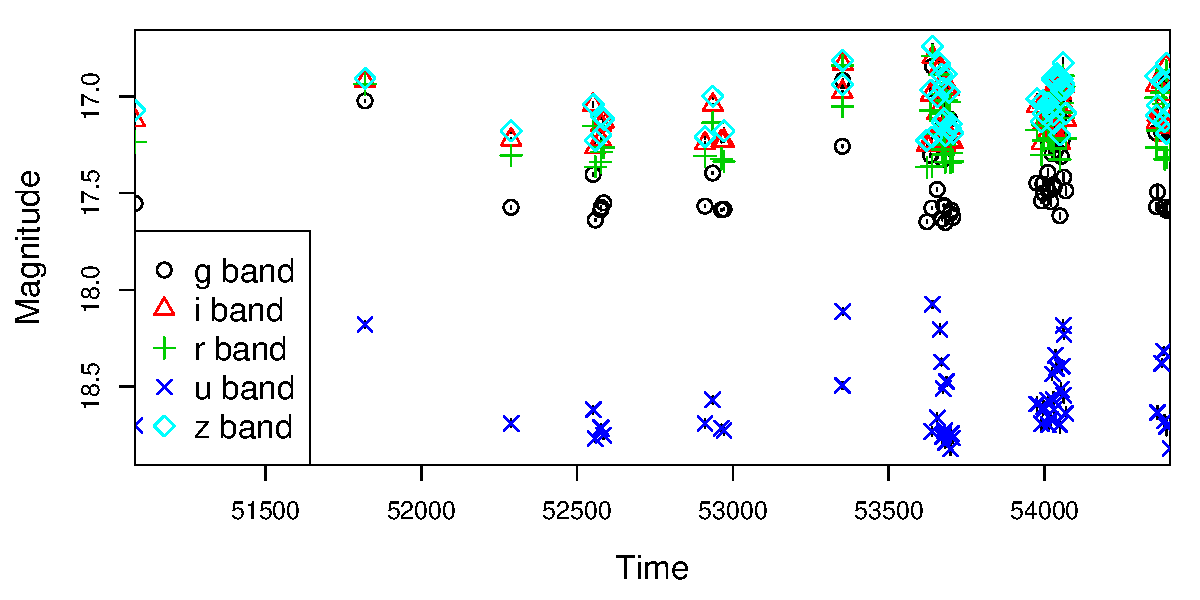
\includegraphics[scale=.4]{figs/unfolded.pdf}
\end{center}
\begin{itemize}
\item Star observed $n=367$ times.
\item Data for star is $D=\{t_i,m_i,\sigma_i\}_{i=1}^n$.
\begin{itemize}
\item Observe star brightness $m_i$ at time $t_i$ with uncertainty $\sigma_i$.
\end{itemize}
\end{itemize}
\end{frame}


\begin{frame}{Folded Light Curve of Periodic Variable}
\textbf{Folded light curve:} Brightness versus time modulo period.
\begin{center}
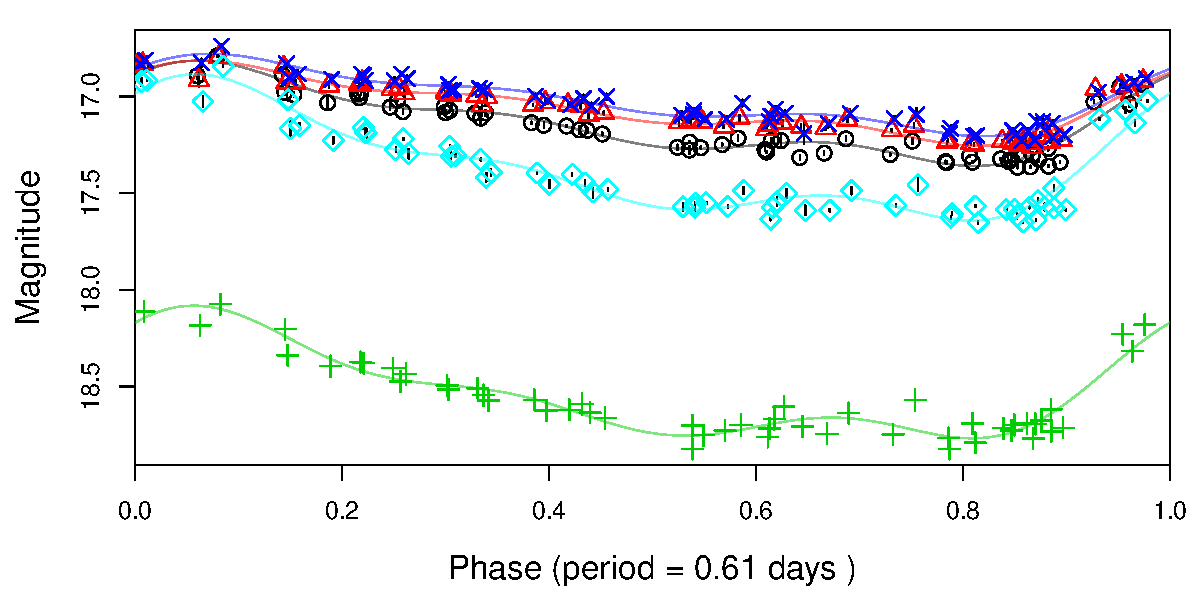
\includegraphics[scale=.4]{figs/folded.pdf}
\end{center}
\end{frame}


\begin{frame}{The OGLE III Survey \cite{udalski2008optical}}
\begin{itemize}
\item Collected 100,000s periodic variables in Large Magellanic Cloud
\item Periodic variables belong to different \textbf{classes}
\item Class is related to astrophysical reason for variation
\end{itemize}

\underline{Two Examples}
\begin{center}
Mira Variable\\
\includegraphics[scale=.2]{figs/mira1_unfolded.pdf}
\includegraphics[scale=.2]{figs/mira1_folded.pdf}
\end{center}

\vspace{.1in}

\begin{center}
RR Lyrae AB Variable\\
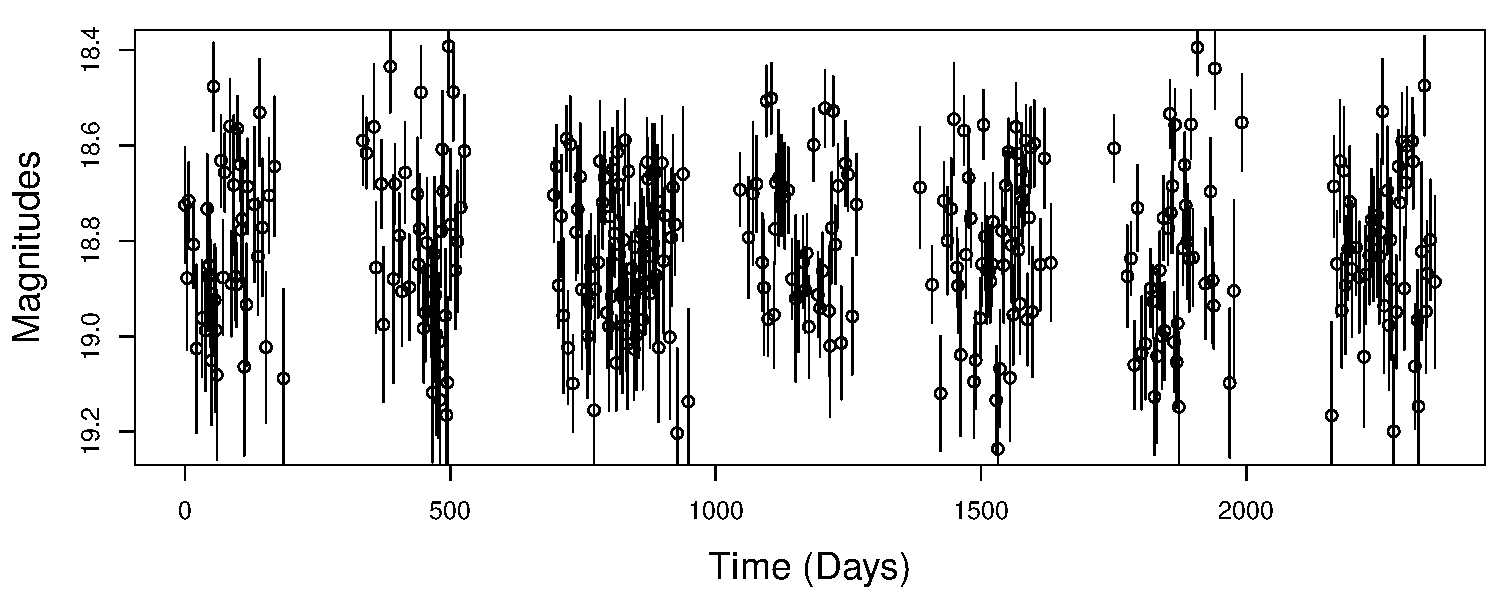
\includegraphics[scale=.2]{figs/rra_unfolded.pdf}
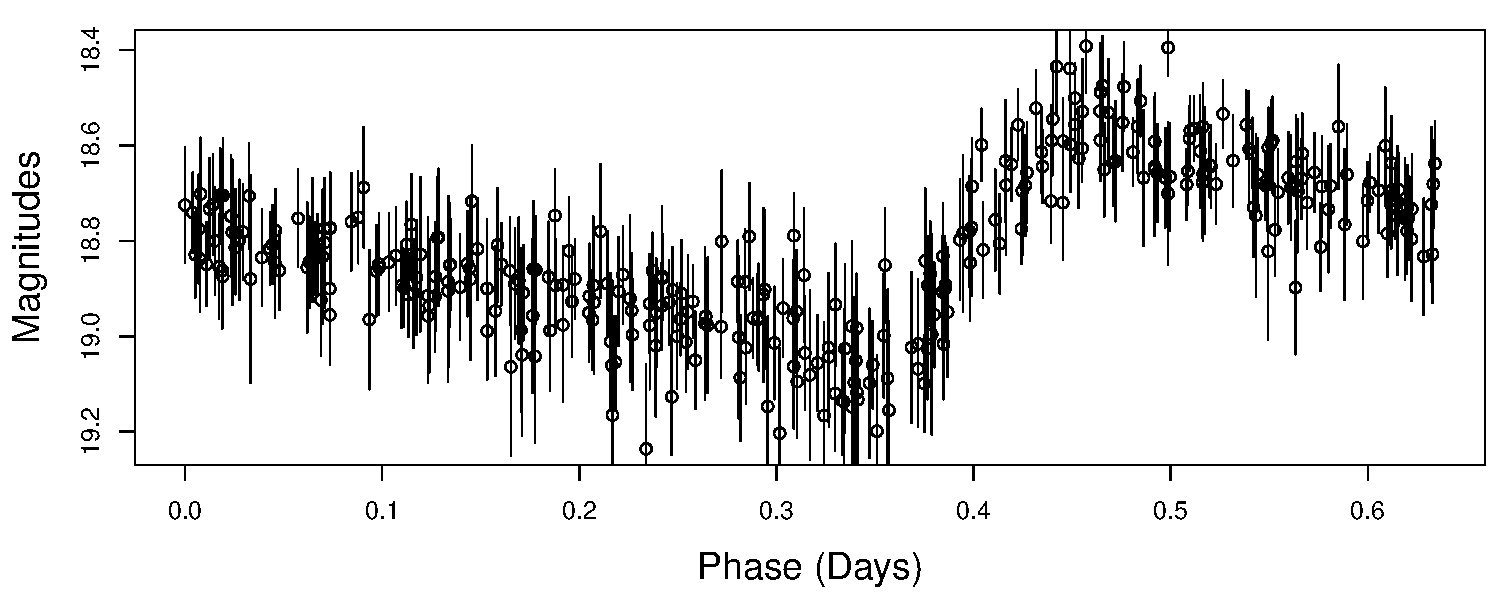
\includegraphics[scale=.2]{figs/rra_folded.pdf}
\end{center}

\end{frame}


\begin{frame}{Size of Variable Star Data Sets is Growing}
\begin{itemize}
\item \textit{Hipparcos} (1989--1993): 2712 
\item \textit{OGLE} (1992--present): 100,000s
\item \textit{DES} (ongoing): $\sim$ 10 million
\item \textit{LSST} (starting 2020): $\sim$ 1 billion

\vspace{.4in}

Data sets of varying quality:
\begin{center}
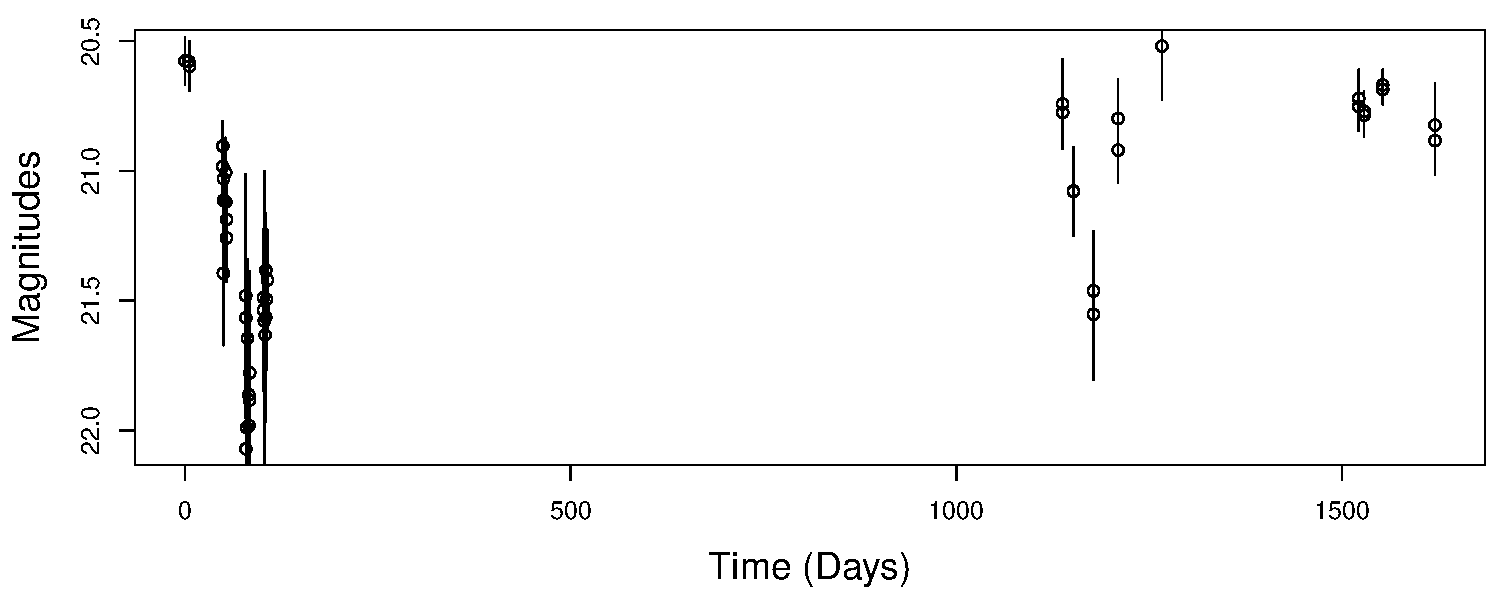
\includegraphics[scale=.3]{figs/m33_unfolded.pdf}
\end{center}


\end{itemize}

%\textbf{Dramatic Differences in Data Quality:}

\end{frame}



%%%%%%%%
%%%%%%%% TODO: discuss panstarrs / DES, performance of lomb scargle
%%%%%%%%

\section{Pan--STARRS and Lomb Scargle}

%%%%%%%%
%%%%%%%% TODO: introduce model, discuss fitting
%%%%%%%%


\section{Parsimoneous Model for RR Lyrae Variables}

\section{Conclusions and Future Work}

\begin{frame}{Folded Light Curve using Two Sinusoidal Models}
\begin{center}
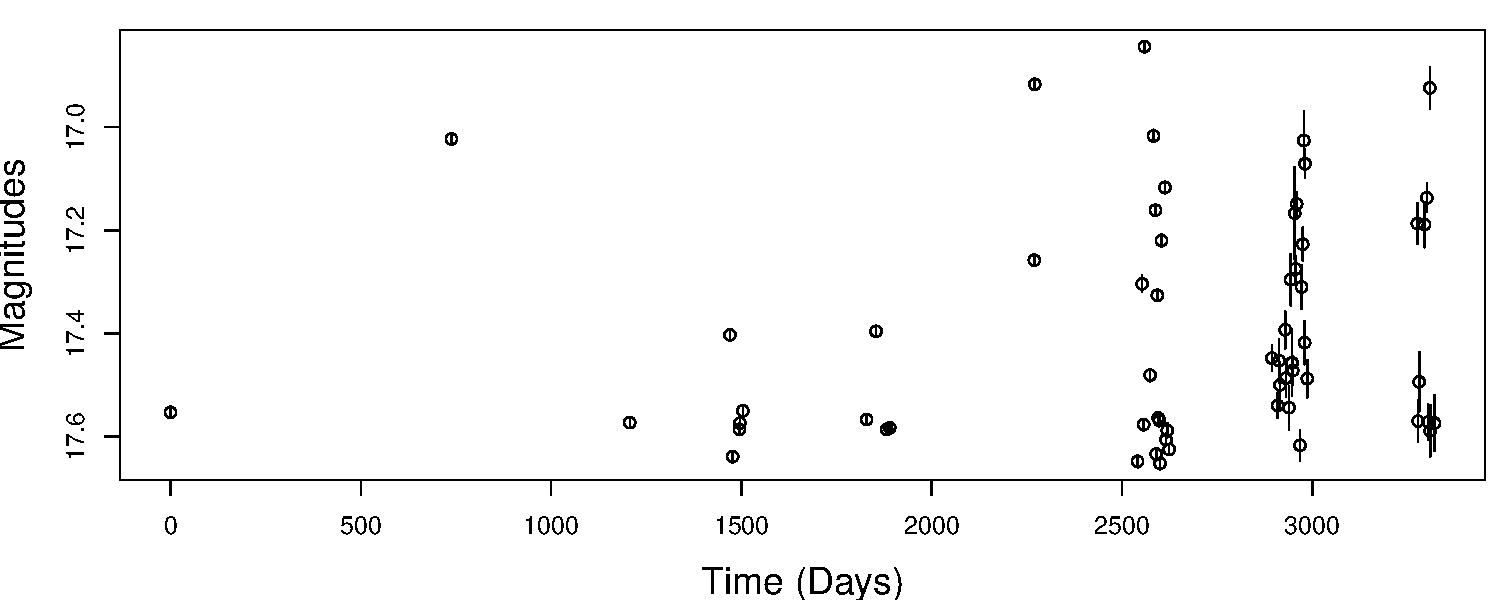
\includegraphics[scale=0.32]{figs/unfolded_single.pdf}\\
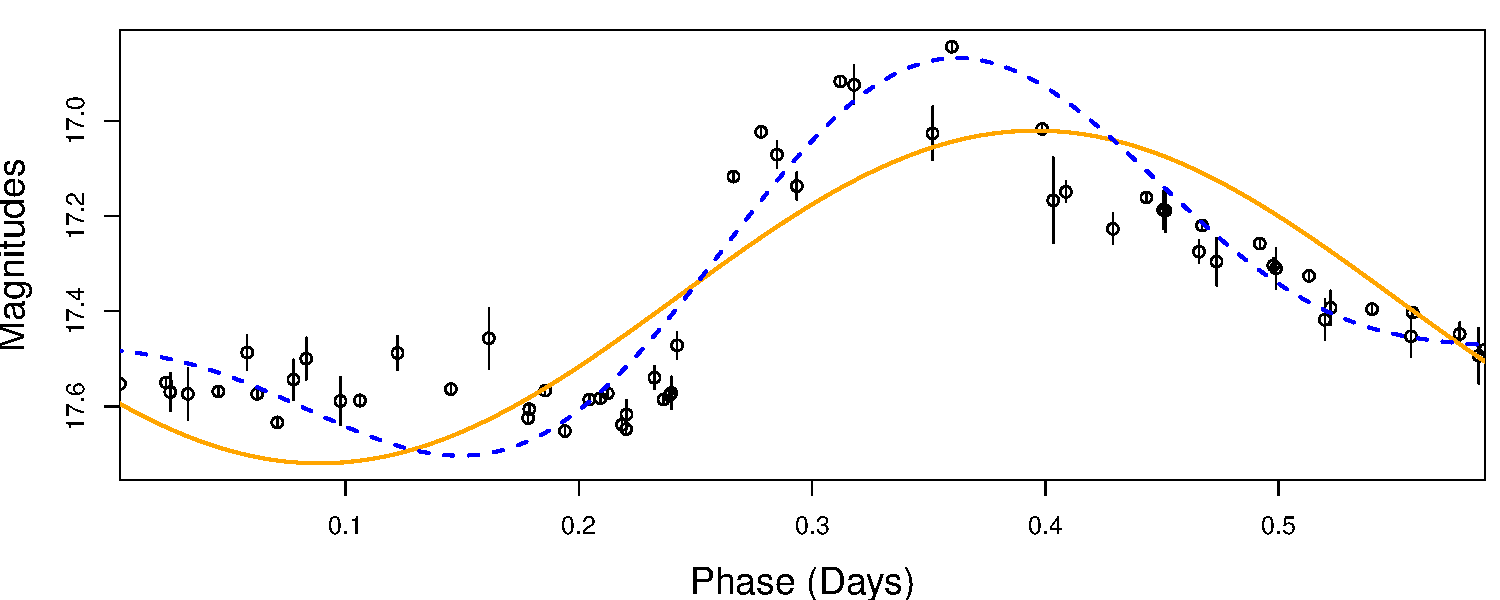
\includegraphics[scale=0.32]{figs/folded_single.pdf}
\end{center}
\end{frame}

\begin{frame}{Period Estimation for Variable Stars}
\textbf{Common Model:} 
\begin{equation*}
m_i = \beta_0 + \sum_{k=1}^K a_k \sin(t_i\omega k + \phi_k) + \epsilon_i
\end{equation*}
where $\epsilon_i \sim N(0,\sigma_i^2)$ {\tiny Zechmeister \cite{zechmeister2009generalised}, Schwarzenberg \cite{schwarzenberg1996fast}}

\vspace{.2in}

\textbf{Maximum likelihood estimator:}
\begin{equation*}
\widehat{\omega} = \argmin{\omega} \min_{\phi,a,\beta_0} \sum_{i=1}^n\left(\frac{m_i - \beta_0 - \sum_{k=1}^K a_k\sin(\omega t_ik + \phi_k)}{\sigma_i}\right)^2
\end{equation*}
\end{frame}



\begin{frame}{Question}
\begin{itemize}
\item Misspecified models are common and can be useful.
\item Heteroskedasticity in responses is common.
\item Typically we weight observations by inverse of variance.
\end{itemize}

\vspace{.3in}
\textbf{Question:} Is this weighting helpful when the model is misspecified?

\end{frame}


%% \begin{frame}{Example: Period Estimation for Variable Stars}
%% \begin{center}
%% 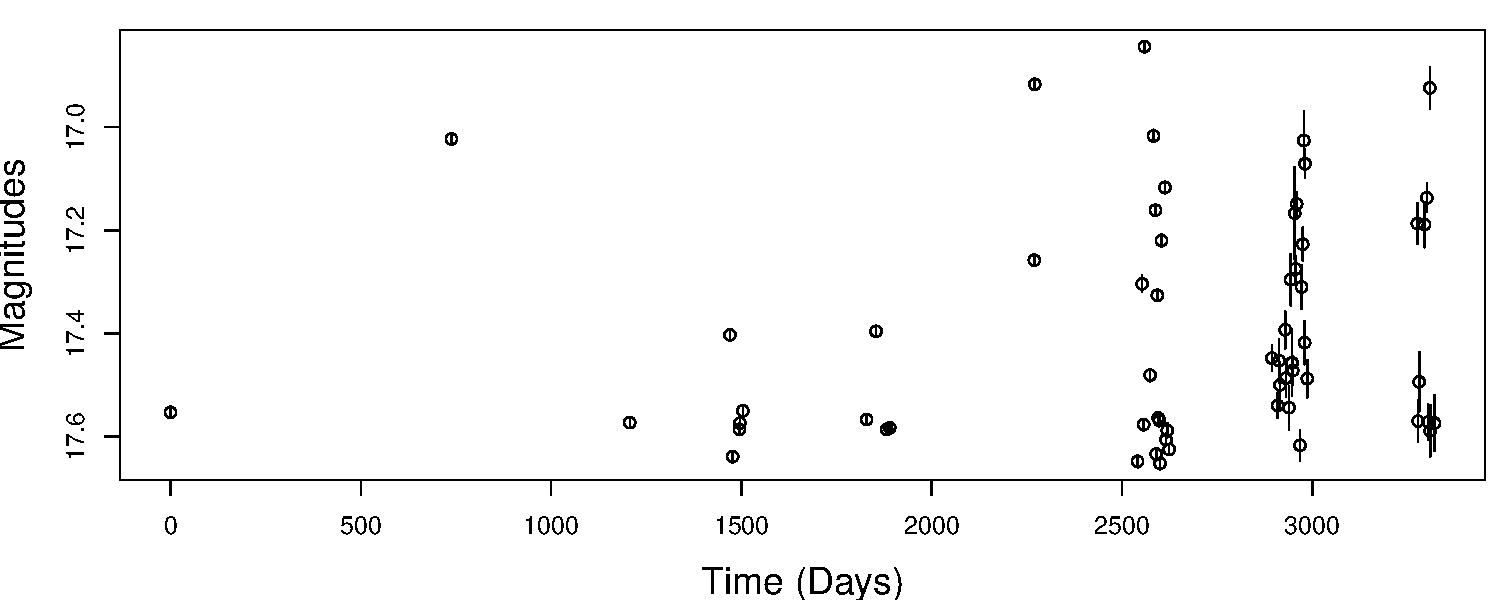
\includegraphics[scale=0.35]{figs/unfolded_single.pdf}
%% \end{center}
%% \textbf{Data:} $D = \{(t_i,m_i,\sigma_i)\}_{i=1}^n$
%% \begin{itemize}
%% \item magnitude $m_i$
%% \item observed at time $t_i$
%% \item with uncertainty $\sigma_i$
%% \end{itemize}
%% \vspace{.2in}
%% \textbf{Goal:} Estimate period, amplitude, etc. of star.
%% \end{frame}

%% \begin{frame}{hello}
%% \cite{zechmeister2009generalised}
%% \end{frame}



%% \begin{frame}{Simulate a sinusoidal light curve}
%%  % with $K=1$, $p = 2\pi / \omega = 1$, $a = 1$, $\beta_0 = 14$, $\beta_0 = 14$, $\sigma_i = 0.3$.

%% \begin{center}
%% \includegraphics[scale=.5]{code/figs/lc_sine.pdf}
%% \end{center}

%% \end{frame}

%% \begin{frame}{Correct Model}
%% \begin{center}
%% \includegraphics[scale=.5]{code/figs/sd1.pdf}
%% \end{center}
%% \end{frame}

%% \begin{frame}{Correct Model}
%% \begin{center}
%% \includegraphics[scale=.5]{code/figs/sd2.pdf}
%% \end{center}
%% \end{frame}

\begin{frame}{Correct Model: Weighted Fit}
\begin{center}
\includegraphics[scale=.5]{code/figs/sd3.pdf}
\end{center}
\end{frame}

\begin{frame}{Correct Model: Unweighted Fit}
\begin{center}
\includegraphics[scale=.5]{code/figs/sine_unweight.pdf}
\end{center}
\end{frame}


%% \begin{frame}{Correct Model}
%% \begin{center}
%% \includegraphics[scale=.5]{code/figs/sd5.pdf}
%% \end{center}
%% \end{frame}



\begin{frame}{Summary}
\begin{itemize}
\item The fitted curve (orange line) is close to observations with small  error (small $\sigma_i$).
\item This is good \textbf{when the actual light curve variation is sinusoidal.}
\end{itemize}

\vspace{.2in}
\textbf{Question:} What happens for misspecified models (light curves that are not actually sinusoids)?

\end{frame}


%% \begin{frame}{Simulate negative sawtooth (RR Lyrae like shape)}
%%  % with $K=1$, $p = 2\pi / \omega = 1$, $a = 1$, $\beta_0 = 14$, $\beta_0 = 14$, $\sigma_i = 0.3$.

%% \begin{center}
%% \includegraphics[scale=.5]{code/figs/lc_sawtooth.pdf}
%% \end{center}

%% \end{frame}



%% \begin{frame}{Misspecified Model -- Weighted Fit}
%% \begin{center}
%% \includegraphics[scale=.5]{code/figs/sd1wrong.pdf}
%% \end{center}
%% \end{frame}

%% \begin{frame}{Misspecified Model -- Weighted Fit}
%% \begin{center}
%% \includegraphics[scale=.5]{code/figs/sd2wrong.pdf}
%% \end{center}
%% \end{frame}

\begin{frame}{Misspecified Model -- Weighted Fit}
\begin{center}
\includegraphics[scale=.5]{code/figs/sd3wrong.pdf}
\end{center}
\end{frame}

\begin{frame}{Misspecified Model -- Unweighted Fit}
\begin{center}
\includegraphics[scale=.5]{code/figs/sd_unweight.pdf}
\end{center}
\end{frame}








\begin{frame}{Application to Variable Star Period Estimation}
\begin{itemize}
\item g--band light curves of 238 bright sources in Stripe 82 SDSS-III
\item Downsampled all light curves to 10,20,30, and 40 observations
\begin{itemize}
\item Simulates difficult period recovery settings encountered by PanStarrs, DES
\end{itemize}
\item Compare period estimation using weighted, unweighted estimators
\end{itemize}
\end{frame}


\begin{frame}{Results}
Fraction of periods estimated correctly for different models ($K=1,2,3$) and using weights ($\Sigma^{-1}$) and unweighted ($I$).

\begin{table}[ht]
\centering
\begin{tabular}{c|cc|cc|cc}
 &   $K=1$ &    & $K=2$ &    & $K=3$ &  \\ 
  \hline
n & $\Sigma^{-1}$ &  $I$ & $\Sigma^{-1}$ &  $I$ & $\Sigma^{-1}$ &  $I$ \\
  \hline10&0.09&0.16&0.13&0.11&0.03&0.03\\20&0.46&0.58&0.63&0.68&0.69&0.77\\30&0.64&0.78&0.71&0.82&0.82&0.86\\40&0.75&0.79&0.80&0.85&0.87&0.92\\\hline
\end{tabular}
\caption{Fraction of periods estimated correctly (within 1\%) using models with $K=1,2,3$ harmonics ($p=4,5,8$ parameters, respectively). Ignoring the observation uncertainties ($I$) in the fitting is superior to using them ($\Sigma^{-1}$). The standard deviation on these accuracies is no larger than $\sqrt{0.5(1-0.5)/238} \approx 0.032$ .}
\label{tab:period_est_results}
\end{table}


\vspace{.1in}
\textbf{Conclusion:} Ignoring heteroskedasticity can improve model fits.
\end{frame}

\begin{frame}{Notes}
%% 1. $\Delta$ idea
%% 2. link to paper
\begin{itemize}
\item linear model case:
\begin{align*}
x_i &\sim f_X, \, \, \, \sigma_i \sim f_\sigma, \, \, \, \sigma_i \indep x_i\\
y_i &= f(x_i) + \epsilon_i \text{ where } \epsilon_i \sim N(0,\sigma_i^2)\\
\beta &\equiv \argmin{\beta} \E[(f(x) - x^T\beta)^2] = \E[xx^T]^{-1}\E[xf(x)].
\end{align*}
$\widehat{\beta} = (X^T\Sigma^{-1}X)^{-1}X^T\Sigma^{-1}Y$ not efficient.
\item Adaptively choose optimal weights: $(\sigma_i^2 + \Delta)^{-1}$
\item close connections with Y. Ma \cite{ma2006efficient,ma2013doubly}
\item many more details: ``Parameter Estimation for Misspecified Regression Models with Heteroskedastic Errors'' \url{http://arxiv.org/abs/1509.05810}
\end{itemize}
\end{frame}



\section{Period Estimation and Classification for M33 Miras}

\begin{frame}{Collaboration}
%% astronomers
  \begin{textblock*}{12cm}(0cm,1cm) % {block width} (coords)
\begin{center}
\textbf{Astronomy}
\end{center}
\end{textblock*}
  \begin{textblock*}{3cm}(3.5cm,2cm) % {block width} (coords)
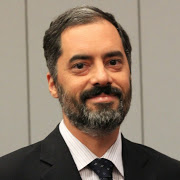
\includegraphics[width=\w,height=\h]{figs/Macri.jpg}\\
Lucas Macri
\end{textblock*}
  \begin{textblock*}{3cm}(7cm,2cm) % {block width} (coords)
\includegraphics[width=\w,height=\h]{figs/yuan.jpg}\\
Wenlong Yuan
\end{textblock*}


%% statisticians
  \begin{textblock*}{12cm}(0cm,5.1cm) % {block width} (coords)
\begin{center}
\textbf{Statistics}
\end{center}
\end{textblock*}

  \begin{textblock*}{3cm}(1.5cm,6.1cm) % {block width} (coords)
\includegraphics[width=\w,height=\h]{figs/he.jpg}\\
Shiyuan He
\end{textblock*}


  \begin{textblock*}{3cm}(5cm,6.1cm) % {block width} (coords)
\includegraphics[width=\w,height=\h]{figs/Huang2.jpg}\\
Jianhua Huang
\end{textblock*}

  \begin{textblock*}{3cm}(8.5cm,6.1cm) % {block width} (coords)
\includegraphics[width=\w,height=\h]{figs/long2.jpg}\\
James Long
\end{textblock*}
\end{frame}


\begin{frame}{Period Luminosity Relation for Miras in the LMC}


%% \begin{textblock*}{3cm}(8cm,1.5cm) % {block width} (coords)
%% \includegraphics[scale=.25]{figs/lmc2.jpg}\\
%% \end{textblock*}

\begin{textblock*}{3cm}(1cm,1.5cm) % {block width} (coords)
\includegraphics[scale=.25]{figs/lmc2.jpg}
\end{textblock*}




\begin{textblock*}{3cm}(6cm,1.5cm) % {block width} (coords)
\includegraphics[scale=.22]{figs/period_luminosity_miras.pdf}
\end{textblock*}



\begin{textblock*}{3cm}(3cm,5.5cm) % {block width} (coords)
\includegraphics[scale=.25]{figs/mira1_unfolded.pdf}\\
\end{textblock*}


\end{frame}


\begin{frame}{PL Relation for Miras in M33}

\begin{textblock*}{3cm}(8cm,2.5cm) % {block width} (coords)
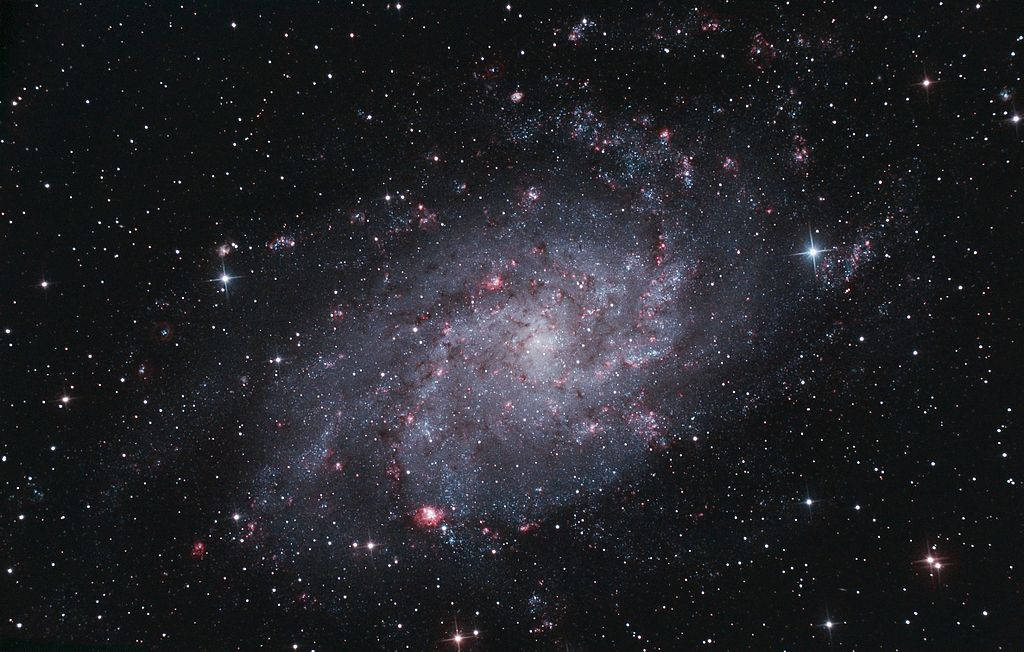
\includegraphics[scale=.1]{figs/m33.jpg}
\end{textblock*}




\textbf{Estimating PL Relation requires:}



\begin{itemize}
\item Estimating periods and luminosities accurately.
\item Classifying stars.
\end{itemize}


\vspace{.3in}

\textbf{Challenging case:}
\begin{center}
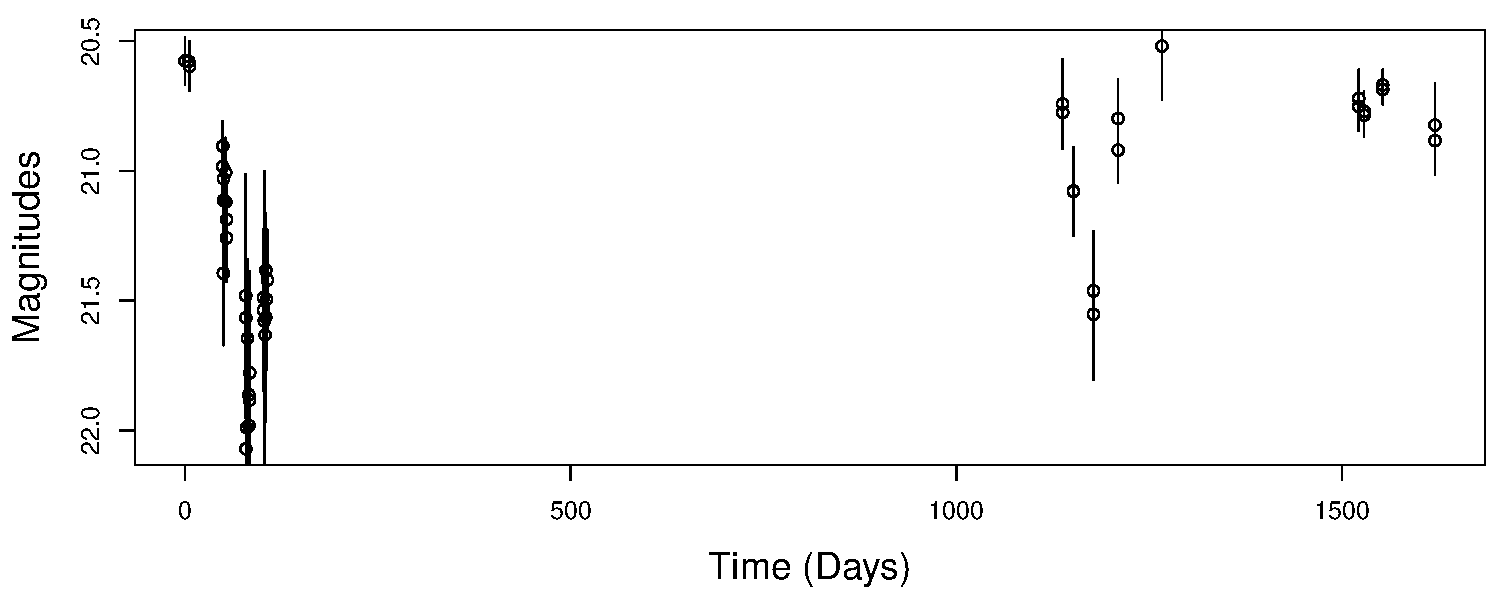
\includegraphics[scale=.4]{figs/m33_unfolded.pdf}
\end{center}

\end{frame}


\begin{frame}{Sinusoid Fit to LMC Mira}

\begin{center}
\includegraphics[scale=.3]{figs/mira4_unfolded_fit.pdf}\\
\includegraphics[scale=.3]{figs/mira4_folded_fit.pdf}
\end{center}

\end{frame}


\begin{frame}{Fit to M33 Mira}

\begin{center}
\includegraphics[scale=.3]{figs/m33_unfolded_fit.pdf}\\
\includegraphics[scale=.3]{figs/m33_folded_fit.pdf}
\end{center}

\vspace{.05in}

Improve sinusoidal model to accurately estimate periods with M33.

\end{frame}


\begin{frame}{Gaussian Process Fit to OGLE Mira}
\begin{center}
\includegraphics[scale=.4]{figs/mira3_GP.pdf}
\end{center}

%% \begin{align*}
%% \widehat{\theta}_{1} &= 1.4\\
%% \widehat{\beta}_{1} &= 1.4\\
%% \widehat{\beta}_{2} &= 2.4\\
%% \end{align*}
\end{frame}


\begin{frame}{Bayes Factors for Separating Different Classes}
\begin{center}
\includegraphics[scale=0.2]{figs/bayes_factor.png}
\end{center}
\end{frame}


\begin{frame}[allowframebreaks]{Bibliography}
%  \def\newblock{\hskip .11em plus .33em minus .07em}
%  \nocite{*}
%\nocite{*}
\bibliographystyle{plain} 
  \tiny{
  \bibliography{refs}}
\end{frame}

\end{document}


